%
% Perspective
%

% !TEX root = ../../main.tex

\chapter{Diskussion und Ausblick\label{chap:perspective}}

  \todo[inline]{Bespricht die erzielten Ergebnisse bezüglich ihrer Erwartbarkeit, Aussagekraft und Relevanz}
  \todo[inline]{Interpretation und Validierung der Resultate}
  \todo[inline]{Rückblick auf Aufgabenstellung, erreicht bzw\@. nicht erreicht}
  \todo[inline]{Legt dar, wie an die Resultate angeschlossen werden kann; legt dar, welche Chancen die Resultate bieten}

  \section{Diskussion der Resultate\label{sec:diskRes}}

    Die gefundenen Resultate wiederspiegeln Lösungen innerhalb einer künstlichen Umgebung.
    In dieser Umgebung wird eine vereinfachte Physik verwendet, welche nur eine Annäherung and die reale Physik ist.
    Deshalb sind die Resultate nicht ohne Vorbehalte auf die reale Welt übertragbar.
    \\
    Das Evolvieren von artifiziellen Tieren und ihrer Steuerung ist möglich
    mit dem implementierten evolutionären Algorithmus.
    Es entwickelte sich keine klassische Laufbewegung,
    aber eine Bewegung welche es den Individuen erlaubt sich durch den Parcours fortzubewegen.
    \\
    Es stellt sich heraus, dass eine Simulation viel Zeit beansprucht und äusserst rechenintensiv ist.
    12000 Generationen zu simulieren, dauert rund 10 Tage.
    \\
    Es kann die Hypothese aufgestellt werden, dass die JavaScript-Engine V8 momentan noch nicht ausreichend schnell ist.
    Eine weiterführende Arbeit könnte untersuchen wie die Leistungen anderer Implementationen von Javascript-Engines im
    Vergleich zu V8 abschneiden.

    \subsection{Wie kann eine Steuerung der Bewegung implementiert werden?}

      Wie in~\vref{sec:Engine} beschrieben ist die Steuerung der Bewegung ist in zwei Teile aufgeteilt.
      Einerseits die Daten im Genotyp und andererseits in die Logik, der Motor.
      Es existiert nur ein Bewegungsablauf pro Individuum.
      Damit wird erreicht, dass keien Synchronisation zwischen mehreren Motoren stattfinden muss.
      Was wiederum die Komplexität des Motors reduziert.

      \smallskip

      Die Aufteilung bietet mehrere Vorteile.
      Die Implementation des Motors und der Mutation des Bewegungsablaufs kann getrennt werden.
      Die Mutation verarbeitet nur die Repräsentation des Bewegungsablaufs.
      Innerhalb der Mutation muss deshalb nur die Struktur der Daten bekannt sein.
      Vorteilhaft für die Implementation des Motors ist, dass dieser nur den vorgegebenen Ablauf abarbeiten muss.

      \smallskip

      Ein Nachteil der Implementation des Motors ist, dass das Feedback-System nicht trivial implementiert werden kann.
      Der Motor muss anhand des Feedbacks entscheiden, was weiter geschehen soll.
      Für jede Kombination von Zustand des Bewegungsablaufs und Art des Feedbacks muss definiert werden,
      was der nächste Zustand des Motors sein muss.
      Zustände werden währen der Evolution erstellt und gelöscht.
      Somit müssen diese Regeln dynamisch erstellt werden können.

      \smallskip

      Die erzielten Resultate mit der Implementation des Motors sind zufriedenstellend.
      In der gegebenen Form werden Bewegungsmuster entwickelt, die an den Parcours angepasst werden.
      Es gilt zu beachten, dass diese Resultate unter dem von Floreano~\cite{Floreano2010} beschriebenen Problem
      der evolutionären Robotik leiden.
      Die entwickelten Individuen nutzen an bestimmten Stellen Eigenschaften des Parcours aus.
      Eigenschaften innerhalb eines Parcours sind besondere Geländeformationen.
      Damit lässt sich herleiten,
      weshalb Simulationen mit einer höheren Wahrscheinlichkeit für das Hinzufügen von Bewegungen als das Löschen
      bessere Resultate liefern.
      Mit den zusätzlichen Bewegugnen kann das Individuum seinen Bewegungsablauf
      an weitere Geländeformationen adaptieren und erreicht somit eine höhere Fitness.

      % TODO 1200 gen

      TEXT~\vref{sub:PerspectiveFeedback}.

    \subsection{Wie kann diese Steuerung evolviert werden?}

      Damit die Steuerung der Bewegung, der Bewegungsablauf, evolviert werden kann,
      muss dieser in einer Form vorliegen, die es erlaubt einzelne Werte zu manipulieren.
      Der Bewegungsablauf beinhaltet eine Liste von Bewegungen.
      In der Liste können Bewegungen beliebig gruppiert werden.
      Wie in~\vref{subsub:EngineMovement} beschrieben
      wird die Information zu einer Bewegung in mehrere Teile aufgespaltet.
      Die gewählte Darstellungsform bietet eine fein gegliederte Beschreibung des Bewegungsablaufs.
      Diese Gleiderung erlaubt es den Bewegungsablauf einfach zu entwickeln.
      \\
      Der Bewegungsablauf ist hauptverantwortlich für die Fitness eines Individuums.
      Dies führt dazu, dass Individuen mit einem ausgereiften Bewegungsablauf mit grösserer Wahrscheinlichkeit
      für die Reproduktion selektiert und anschliessen mutiert werden.
      \\
      % TODO moaaar

    \subsection{Wie kann die Geometrie der Tiere evolviert werden?}

      Die Konstruktion der geometrischen Körper aus denen sich ein Individuum zusammensetzt,
      wurde unter~\vref{sub:Beine} und~\vref{subsub:GenotypeBodypointCreation} besprochen.
      Welche Geometrie die richtige ist, wird durch die Selektion und Mutation der Individuen bestimmt.

    \subsection{Nimmt die Diversität mit zunehmenden Generationen stetig ab?}

      Analysiert man die Diversitätsgraphe aus dem vierten~(\vref{sec:4lauf}) und
      fünften Simmulationslauf~(\vref{sec:5lauf}) sieht man einen Abfall der Diversität in den ersten Generationen.
      Bei der allgemeinen Lösung erholt sich die Diversität mit zunehmenden Generationen.
      Gewisse Ausreisser erreichen sogar die Diversität der ersten Generationen.
      Jedoch zeichnet sich ein anderes Bild bei dem Evolvieren auf Evolvierbarkeit ab.
      Hier fällt die Fitness ab der 2000. Generation auf ein niedriges Niveau.
      Es hat sich gezeigt, dass die allgemeine Lösung diverse Individuen liefert.

    \subsection{Wie sieht der Bewegungsablauf und Geometrie eines evolvierten Tieres aus?}

      Neben der vordefinierten Bewegungsablauf~(\vref{sec:Engine}) wurden drei weitere Typen gefunden:

      \begin{itemize}
        \item Rollbewegung
        \item Hüpfbewegung
        \item Ruderbewegung
      \end{itemize}

      Bei der Rollbewegung kippen die Individuen vornüber und drehen sich einmal um sich selber.
      Die Gemoetrie des Körpers tendiert zu einer kreisartigen Form.
      Beine spielen bei dieser Art von Bewegung eine untergeordnete Rolle.

      \begin{figure}[H]
        \centering

        \begin{subfigure}[b]{0.3\textwidth}
          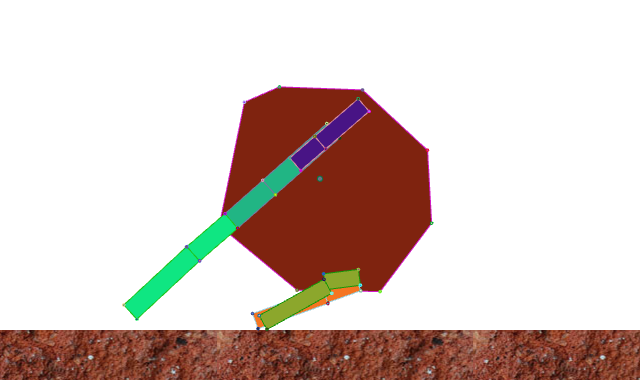
\includegraphics[width=\linewidth,center]{graphics/simulation-discussion/roll_1}
          \caption{\label{fig:roll_1}}
        \end{subfigure}
        \hspace{\fill}
        \begin{subfigure}[b]{0.3\textwidth}
          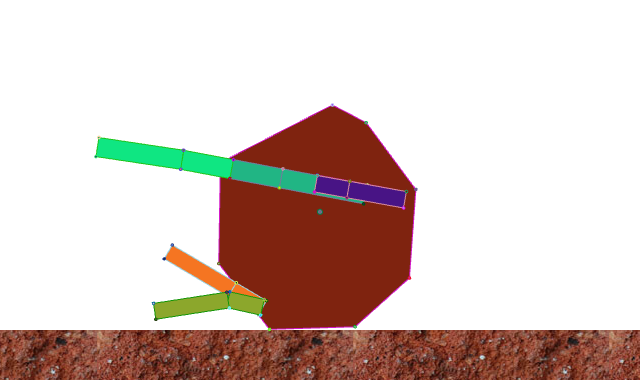
\includegraphics[width=\linewidth,center]{graphics/simulation-discussion/roll_2}
          \caption{\label{fig:roll_2}}
        \end{subfigure}
        \hspace{\fill}
        \begin{subfigure}[b]{0.3\textwidth}
          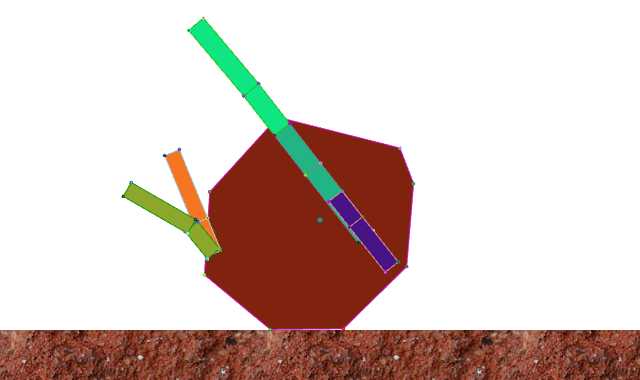
\includegraphics[width=\linewidth,center]{graphics/simulation-discussion/roll_3}
          \caption{\label{fig:roll_3}}
        \end{subfigure}

        \begin{subfigure}[b]{0.3\textwidth}
          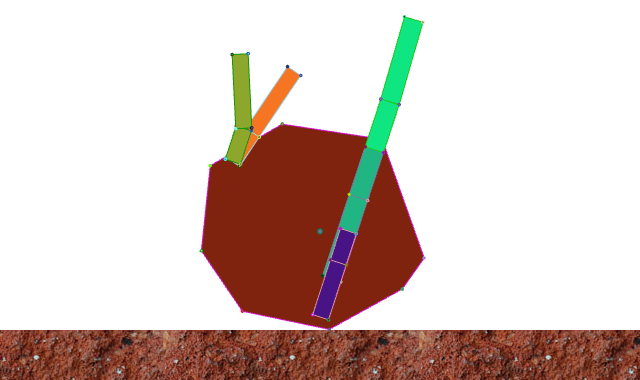
\includegraphics[width=\linewidth,center]{graphics/simulation-discussion/roll_4}
          \caption{\label{fig:roll_4}}
        \end{subfigure}
        \hspace{\fill}
        \begin{subfigure}[b]{0.3\textwidth}
          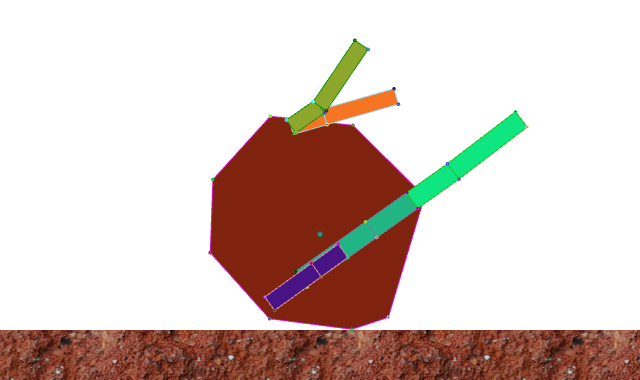
\includegraphics[width=\linewidth,center]{graphics/simulation-discussion/roll_5}
          \caption{\label{fig:roll_5}}
        \end{subfigure}
        \hspace{\fill}
        \begin{subfigure}[b]{0.3\textwidth}
          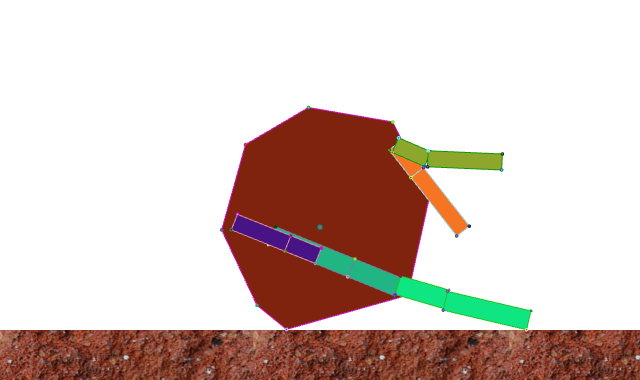
\includegraphics[width=\linewidth,center]{graphics/simulation-discussion/roll_6}
          \caption{\label{fig:roll_6}}
        \end{subfigure}

        \caption{Rollbewegung im Zeitraffer\label{fig:roll}}

      \end{figure}

      Die Hüpfbewegung in~\vref{fig:hupf} führen die Individuen aus, in dem sie sich mit einem Bein vom Boden abstossen.
      Es lässt sich keine Tendenz zu einer bestimmten Körperform erkennen.

      \begin{figure}[H]
        \centering

        \begin{subfigure}[b]{0.3\textwidth}
          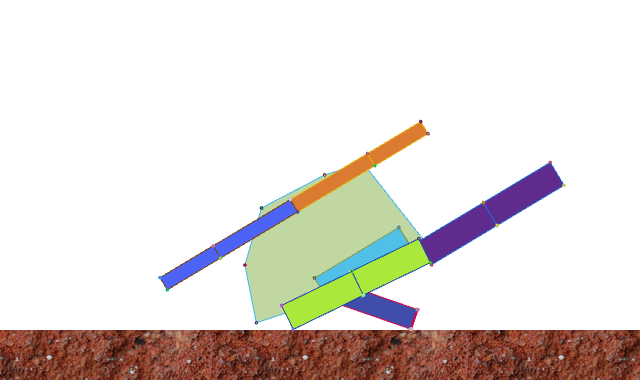
\includegraphics[width=\linewidth,center]{graphics/simulation-discussion/hupf_1}
          \caption{\label{fig:hupf_1}}
        \end{subfigure}
        \hspace{\fill}
        \begin{subfigure}[b]{0.3\textwidth}
          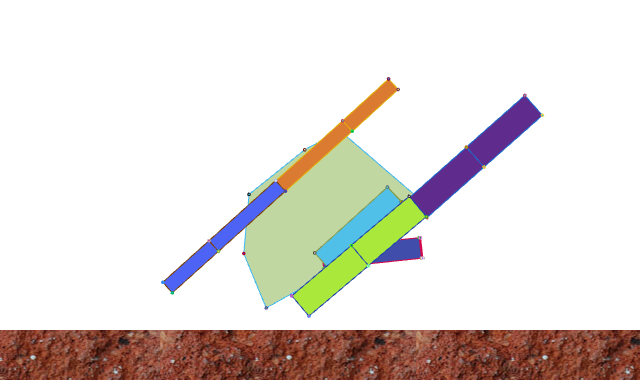
\includegraphics[width=\linewidth,center]{graphics/simulation-discussion/hupf_2}
          \caption{\label{fig:hupf_2}}
        \end{subfigure}
        \hspace{\fill}
        \begin{subfigure}[b]{0.3\textwidth}
          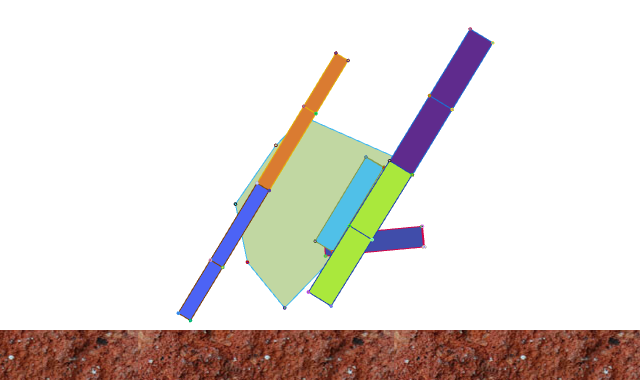
\includegraphics[width=\linewidth,center]{graphics/simulation-discussion/hupf_3}
          \caption{\label{fig:hupf_3}}
        \end{subfigure}

        \begin{subfigure}[b]{0.3\textwidth}
          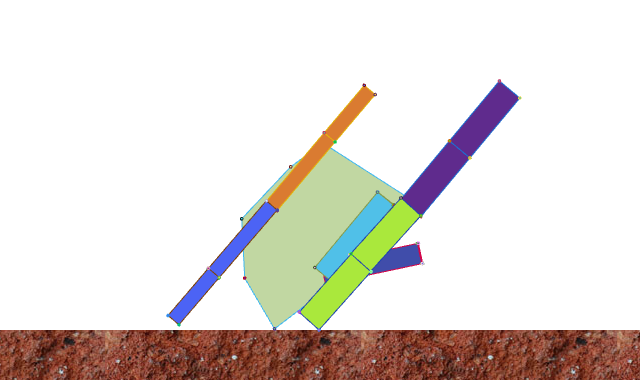
\includegraphics[width=\linewidth,center]{graphics/simulation-discussion/hupf_4}
          \caption{\label{fig:hupf_4}}
        \end{subfigure}
        \hspace{\fill}
        \begin{subfigure}[b]{0.3\textwidth}
          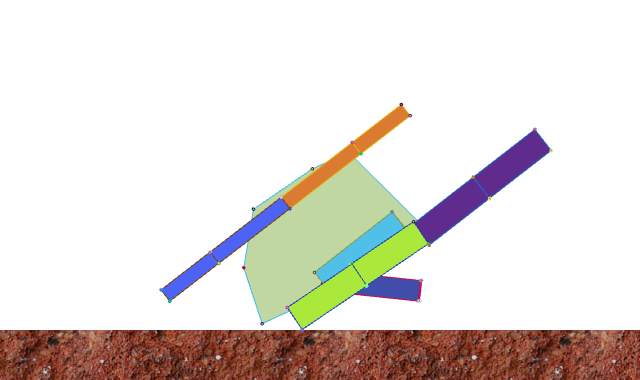
\includegraphics[width=\linewidth,center]{graphics/simulation-discussion/hupf_5}
          \caption{\label{fig:hupf_5}}
        \end{subfigure}
        \hspace{\fill}
        \begin{subfigure}[b]{0.3\textwidth}
          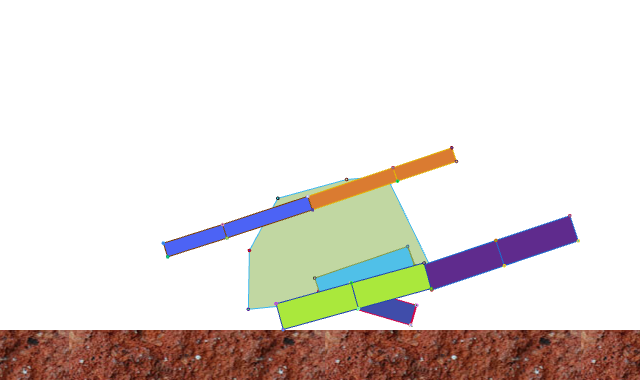
\includegraphics[width=\linewidth,center]{graphics/simulation-discussion/hupf_6}
          \caption{\label{fig:hupf_6}}
        \end{subfigure}

        \caption{Hüpfbewegung im Zeitraffer\label{fig:hupf}}

      \end{figure}

      Die Ruderer in~\vref{fig:ruder} benutzen ein Bein um die Bewegung durchzuführen,
      alle anderen Beine verharren starr am Körper.
      Die Fixierung der anderen Beine haben sie von ihren Vorfahren~(den Hüpfern) geerbt und noch nicht korrigiert.
      Es wäre von Vorteil, wenn sie alle Beine für die Ruderbewegung nutzen würden.
      Die Massen aller Beinpaare, ausser dass sich bewegende, haben sich verkleinert.
      Der Trend bei den Rundern liegt bei flachen Körpern.

      \begin{figure}[H]
        \centering

        \begin{subfigure}[b]{0.3\textwidth}
          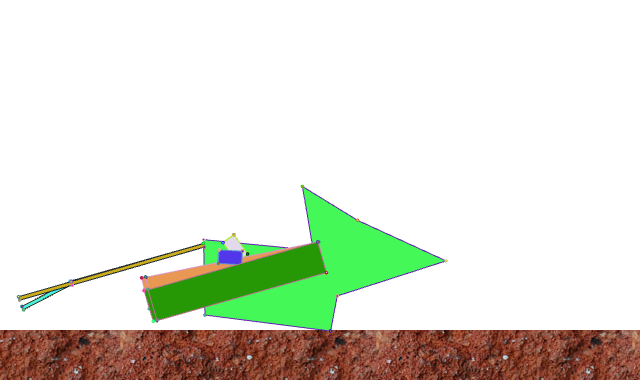
\includegraphics[width=\linewidth,center]{graphics/simulation-discussion/ruder_1}
          \caption{\label{fig:ruder_1}}
        \end{subfigure}
        \hspace{\fill}
        \begin{subfigure}[b]{0.3\textwidth}
          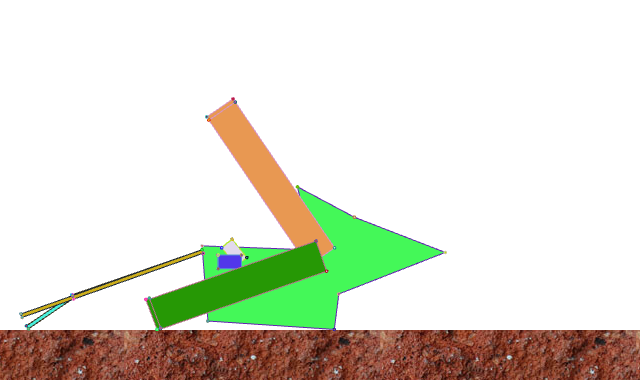
\includegraphics[width=\linewidth,center]{graphics/simulation-discussion/ruder_2}
          \caption{\label{fig:ruder_2}}
        \end{subfigure}
        \hspace{\fill}
        \begin{subfigure}[b]{0.3\textwidth}
          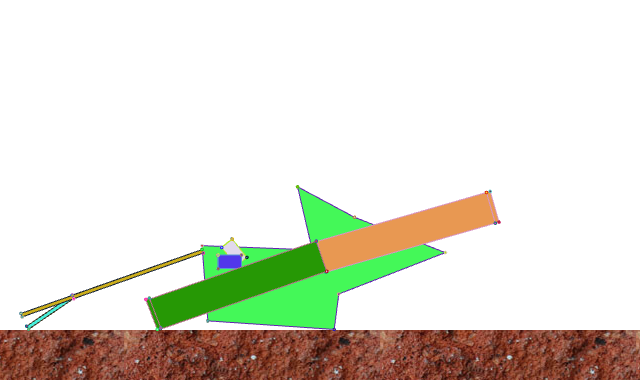
\includegraphics[width=\linewidth,center]{graphics/simulation-discussion/ruder_3}
          \caption{\label{fig:ruder_3}}
        \end{subfigure}

        \begin{subfigure}[b]{0.3\textwidth}
          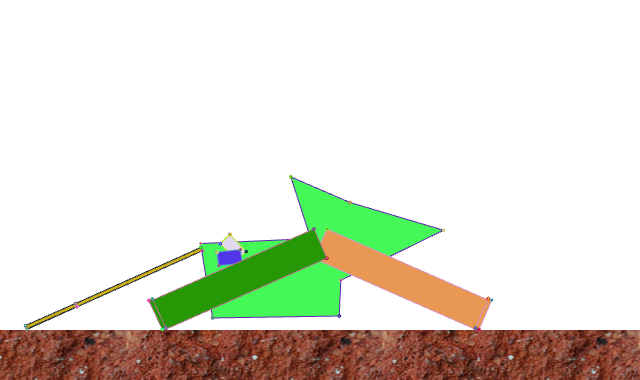
\includegraphics[width=\linewidth,center]{graphics/simulation-discussion/ruder_4}
          \caption{\label{fig:ruder_4}}
        \end{subfigure}
        \hspace{\fill}
        \begin{subfigure}[b]{0.3\textwidth}
          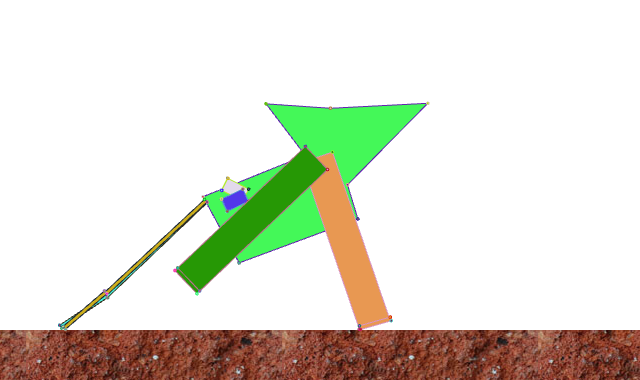
\includegraphics[width=\linewidth,center]{graphics/simulation-discussion/ruder_5}
          \caption{\label{fig:ruder_5}}
        \end{subfigure}
        \hspace{\fill}
        \begin{subfigure}[b]{0.3\textwidth}
          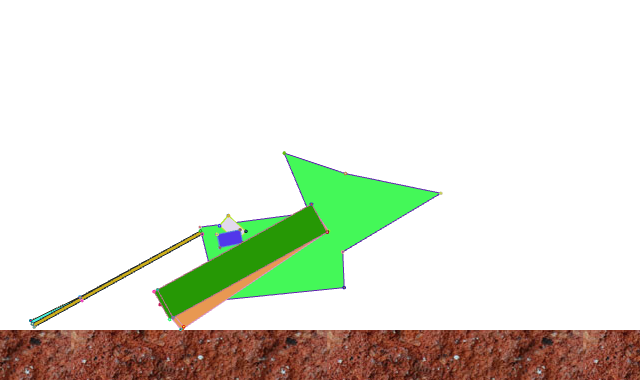
\includegraphics[width=\linewidth,center]{graphics/simulation-discussion/ruder_6}
          \caption{\label{fig:ruder_6}}
        \end{subfigure}

        \caption{Ruderbewegung im Zeitraffer\label{fig:ruder}}

      \end{figure}

    \subsection{Individuum: Allgemeine Lösung vs Evolvieren auf Evolvierbarkeit}

      Es wird das beste Indivdiuum der 4000. Generation~(\vref{fig:gen4000}) aus dem vierten Simulationslauf~\vref{sec:4lauf}
      und dem füften Simulationslauf~(\vref{sec:5lauf}) miteinander verglichen.
      Die Individuen haben beide eine Hüpfbewegung entwickelt.
      Jedoch streckt das eine Individum~(\vref{fig:gen4000_alg}) alle Beine,
      während das Andere~(\vref{fig:gen4000_ev}) fast alle Beine angewinkelt hat.
      Das Strecken der Beine bringt eine bessere Balance,
      dies ist auch der Grund warum das Individum aus der allgemeinen Lösung einen besseren Fitnesswert aufweisen kann.
      Ebenso weisst der Körper des Individuums, welches auf Evolvierbarkeit evolviert wurde, eine grössere Masse auf.
      Die Masse aller Beine ist folglich grösser beim Individum der allgemeinen Lösung.
      Die Steuerung beider Individuen sind also quasi identisch,
      während bei der Geometrie leichte Unterschiede festgestellt worden sind.

      \begin{figure}[H]
        \centering
        \begin{subfigure}[b]{0.45\textwidth}
          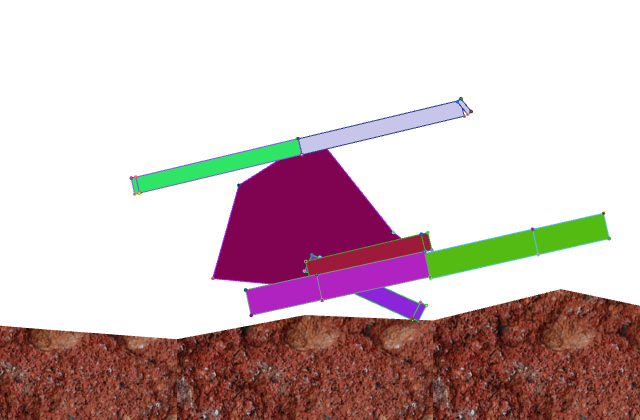
\includegraphics[width=\linewidth,center]{graphics/simulation-discussion/4_gen4000}
          \caption{Allgemeine Lösung\label{fig:gen4000_alg}}
        \end{subfigure}
        \begin{subfigure}[b]{0.45\textwidth}
          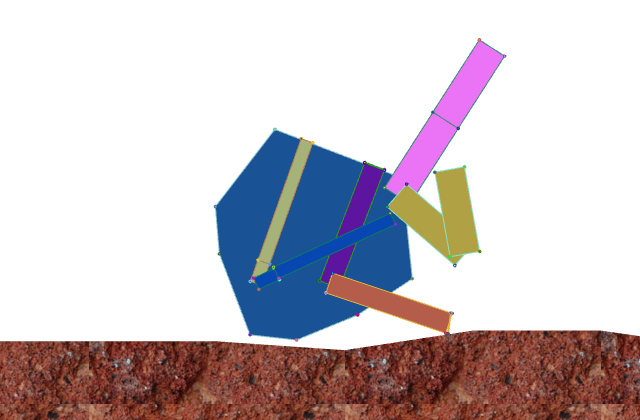
\includegraphics[width=\linewidth,center]{graphics/simulation-discussion/5_gen4000}
          \caption{Evolvierung auf Evolvierbarkeit\label{fig:gen4000_ev}}
        \end{subfigure}

        \caption{4000. Generation\label{fig:gen4000}}
      \end{figure}

      %TODO was heisst das nun?

    \subsection{Hypothese Körperpunkte}

      Um eine Aussage über die Hypothese der Körperpunkte~(\vref{subsub:hypoKp}) zu treffen,
      müsste wie erwähnt unter~\vref{subsub:bpScnd} die Mutation der Anzahl Körperpunkte implementiert werden.
      Spätestens ab der 10. Generation bei jedem Lauf,
      existieren nur noch Individuen mit der gleichen Anzahl Körperpunkten.
      Deshalb kann diese Hypothese nicht validiert werden.

      % TODO validationsstatus konkretisieren

    \subsection{Hypothese Mutationswahrscheinlichkeiten}

      Die Hypothese über die Mutationswahrscheinlichkeiten~(\vref{subsub:hypoMut}) hat sich bewahrheitet
      wie in~\vref{subsub:3000gen} festgestellt worden ist.
      Mit kleineren Mutationswahrscheinlichkeiten lassen sich fittere Indivduen finden.
      % TODO discuss

  \section{Ausblick\label{sec:ausblick}}

    % Tiere mit andere anzahl an beinen als 6

    Die erstellte Simulationsapplikation ist gut erweiterbar und ermöglicht Interessierten sie weiter auszubauen.
    Der Programmcode soll für Interessierte unter \url{http://github.com} freigegeben werden.

    \subsection{Feedback an den Bewegungsmotor\label{sub:PerspectiveFeedback}}

      Die fehlende Implementation der Reaktion auf das Feedback der Steuerung ist sicher die Komponente,
      welche am meisten helfen würde, bessere Resultate zu finden.

    \subsection{Pro Bein ein Bewegungsablauf}
      Momentan beschränkt der definierte Bewegugngsablauf die Individuen auf sechs Beine.
      Wenn auf jedem Bein ein Bewegungsablauf definiert wird, wäre es möglich artifizielle Tiere mit \(n\)-Beinen zu erstellen.
      Es muss aber mit erhöhtem Rechenaufwand gerechnet werden, da die Bewegugnsabläufe miteinander synchronisiert werden müssen.

    \subsection{Austauschen der Physik-Engine}

      Eine Verbesserungsmöglichkeit ist die langsame und teilweise fehlerhafte \gls{PhysicsEngine} p2.js auszutauschen.
      Mit Hilfe einer anderen \gls{PhysicsEngine} kann schneller simuliert werden und
      es können bessere Resultate gefunden werden.
      Für einen 30 Sekunden langen Simulationslauf, benötigt die Engine zum Teil mehr als eine Minute.

    \subsection{Hypothese Selektionsstrategie\label{sub:hypoSelect}}

      Die zeitliche Beschränkung dieser Arbeit hat es nicht erlaubt,
      die ursprünglich geplante Hypothese über den Vergleich von Selektionsstrategien durchzuführen.
      In der Hypothese ging es darum die Auswirkungen von den Selektionsstrategien:
      Turnierbasierte-Selektion, rangbasierte Selektion
      und proportionale Selektion auf die Simulationsresultate zu untersuchen.
      Diese Hypothese würde genügend Stoff für eine weitere spannende Arbeit liefern.

    \subsection{Hypothese Allgemeine Lösung vs.\ Evolvierung auf Evolvierbarkeit\label{sub:hypoAnsatz}}

      Leider war nicht genügend Zeit vorhanden folgende Hypothese zu validieren:
      Individuen welche durch die allgemeine Lösung gefunden werden,
      sollten bei unterschiedlichen Parcours im Durchschnitt besser abschneiden,
      als ihre Gegenspieler~(Evolvierung auf Evolvierbarkeit),
      da sie sich schneller an eine neue Umgebung anpassen können.
      Wenn immer der gleiche Parcours benutzt wird,
      sollten die Individuen welche auf Evolvierbarkeit evolviert worden sind, auf Dauer überlegen sein.
      \\
      Um diese Hypothese zu validieren,
      sollten zwei Simulationsläufe mit zwei Populationen aus den Lösungsansätzen durchgeführt werden:

      \begin{itemize}
        \item Simulationslauf mit gleichem Parcours
        \item Simulationslauf mit 10 unterschiedlichen Parcours
      \end{itemize}

      Anschliessend sollte ein Vergleich angestellt werden zwischen den Lösungsansätzen der beiden Läufen.

    \subsection{Parcours}

      Der Parcours wird nur mit einem Typ von Element generiert, ein Höhenfeld welches einen Berg repräsentiert.
      Neue Terrain-Typen wie Eis, Wasser oder Grass könnten zusätzlich hinzugefügt werden.
      Das Hinzufügen dieser Terrain-Typen würde die Generierung von Individuen zulassen, welche näher an die Realtität herankommen.

      % Tendenz?

    \subsection{Neuronales Netzwerk}

    Der Trend bewegt
      % YEEES
